\PassOptionsToPackage{unicode=true}{hyperref} % options for packages loaded elsewhere
\PassOptionsToPackage{hyphens}{url}
%
\documentclass[british,,man,floatsintext]{apa6}
\usepackage{lmodern}
\usepackage{amssymb,amsmath}
\usepackage{ifxetex,ifluatex}
\usepackage{fixltx2e} % provides \textsubscript
\ifnum 0\ifxetex 1\fi\ifluatex 1\fi=0 % if pdftex
  \usepackage[T1]{fontenc}
  \usepackage[utf8]{inputenc}
  \usepackage{textcomp} % provides euro and other symbols
\else % if luatex or xelatex
  \usepackage{unicode-math}
  \defaultfontfeatures{Ligatures=TeX,Scale=MatchLowercase}
\fi
% use upquote if available, for straight quotes in verbatim environments
\IfFileExists{upquote.sty}{\usepackage{upquote}}{}
% use microtype if available
\IfFileExists{microtype.sty}{%
\usepackage[]{microtype}
\UseMicrotypeSet[protrusion]{basicmath} % disable protrusion for tt fonts
}{}
\IfFileExists{parskip.sty}{%
\usepackage{parskip}
}{% else
\setlength{\parindent}{0pt}
\setlength{\parskip}{6pt plus 2pt minus 1pt}
}
\usepackage{hyperref}
\hypersetup{
            pdftitle={Positive Results in Registered Reports},
            pdfauthor={Anne Scheel, Mitchell Schijen, \& Daniël Lakens},
            pdfkeywords={keyword 1, keyword 2, keyword 3},
            pdfborder={0 0 0},
            breaklinks=true}
\urlstyle{same}  % don't use monospace font for urls
\usepackage{graphicx,grffile}
\makeatletter
\def\maxwidth{\ifdim\Gin@nat@width>\linewidth\linewidth\else\Gin@nat@width\fi}
\def\maxheight{\ifdim\Gin@nat@height>\textheight\textheight\else\Gin@nat@height\fi}
\makeatother
% Scale images if necessary, so that they will not overflow the page
% margins by default, and it is still possible to overwrite the defaults
% using explicit options in \includegraphics[width, height, ...]{}
\setkeys{Gin}{width=\maxwidth,height=\maxheight,keepaspectratio}
\setlength{\emergencystretch}{3em}  % prevent overfull lines
\providecommand{\tightlist}{%
  \setlength{\itemsep}{0pt}\setlength{\parskip}{0pt}}
\setcounter{secnumdepth}{0}
% Redefines (sub)paragraphs to behave more like sections
\ifx\paragraph\undefined\else
\let\oldparagraph\paragraph
\renewcommand{\paragraph}[1]{\oldparagraph{#1}\mbox{}}
\fi
\ifx\subparagraph\undefined\else
\let\oldsubparagraph\subparagraph
\renewcommand{\subparagraph}[1]{\oldsubparagraph{#1}\mbox{}}
\fi

% set default figure placement to htbp
\makeatletter
\def\fps@figure{htbp}
\makeatother

\shorttitle{Positive Results in Registered Reports}
\affiliation{
\vspace{0.5cm}
\textsuperscript{1} Eindhoven University of Technology}
\keywords{keyword 1, keyword 2, keyword 3\newline\indent Word count: XXX}
\usepackage{csquotes}
\usepackage{upgreek}
\captionsetup{font=singlespacing,justification=justified}

\usepackage{longtable}
\usepackage{lscape}
\usepackage{multirow}
\usepackage{tabularx}
\usepackage[flushleft]{threeparttable}
\usepackage{threeparttablex}

\newenvironment{lltable}{\begin{landscape}\begin{center}\begin{ThreePartTable}}{\end{ThreePartTable}\end{center}\end{landscape}}

\makeatletter
\newcommand\LastLTentrywidth{1em}
\newlength\longtablewidth
\setlength{\longtablewidth}{1in}
\newcommand{\getlongtablewidth}{\begingroup \ifcsname LT@\roman{LT@tables}\endcsname \global\longtablewidth=0pt \renewcommand{\LT@entry}[2]{\global\advance\longtablewidth by ##2\relax\gdef\LastLTentrywidth{##2}}\@nameuse{LT@\roman{LT@tables}} \fi \endgroup}


\usepackage{lineno}

\linenumbers
\usepackage{float}
\usepackage{framed}
\usepackage{caption}
\usepackage{setspace}
\captionsetup[textbox]{name=Box,labelsep=period,labelfont=it}
\newfloat{textbox}{thp}{lop}
\floatname{textbox}{Box}
\ifnum 0\ifxetex 1\fi\ifluatex 1\fi=0 % if pdftex
  \usepackage[shorthands=off,main=british]{babel}
\else
  % load polyglossia as late as possible as it *could* call bidi if RTL lang (e.g. Hebrew or Arabic)
  \usepackage{polyglossia}
  \setmainlanguage[variant=british]{english}
\fi

\title{Positive Results in Registered Reports}
\author{Anne Scheel\textsuperscript{1}, Mitchell Schijen\textsuperscript{1}, \& Daniël Lakens\textsuperscript{1}}
\date{}

\authornote{

Correspondence concerning this article should be addressed to Anne Scheel, Den Dolech 1, Atlas 9.417, 5600 MB, Eindhoven, The Netherlands. E-mail: \href{mailto:a.m.scheel@tue.nl}{\nolinkurl{a.m.scheel@tue.nl}}}
\note{\clearpage}
\abstract{
XXXXXXXXXXXXXXXXXXX



}

\begin{document}
\maketitle

\hypertarget{analysis}{%
\subsection{Analysis}\label{analysis}}

We planned to test our hypothesis in the following way (quoting directly from our preregistration, \url{https://osf.io/sy927}, point 9):

\begin{quote}
A one-sided proportion test with an alpha level of \(5\%\) will be performed to test whether the positive result rate (full or partial support) of Registered Reports in psychology is statistically lower than the positive result rate of conventional reports in psychology.
In addition to testing if there is a statistically significant difference between RRs and conventional reports, we will test if the difference is smaller than our smallest effect size of interest using an equivalence test for proportion tests with an alpha level of \(5\%\) (Lakens, Scheel, \& Isager, 2018).
We determined our smallest effect size of interest to be the difference between the positive result rate in psychology (\(91.5\%\)) and the positive result rate in general social sciences (\(85.5\%\)) as reported by Fanelli (2010), i.e.~a difference of \(91.5\% - 85.5\% = 6\%\).
The rationale for choosing general social sciences as a comparison is that this discipline had the lowest positive result rate amongst the \enquote{soft} sciences (Fanelli, 2010).
The exact percentage for general social sciences was extracted from Figure 1 in Fanelli (2010) using the software WebPlotDigitizer (Rohatgi, 2018).
\end{quote}

We would accept our hypothesis that RRs have a lower positive result rate than SRs if we found a negative difference between RRs and SRs that was significantly different from 0 \emph{and} not statistically equivalent to a range from \(-6\%\) to \(+6\%\) (both at \(\alpha = 5\%\)).

\hypertarget{results}{%
\section{Results}\label{results}}

\hypertarget{confirmatory-analyses}{%
\subsection{Confirmatory Analyses}\label{confirmatory-analyses}}

146 out of 152 SRs and 31 out of 71 RRs had positive results, meaning that the positive result rate was \(96.05 \%\) for SRs (\(95 \%\) CI {[}91.61, 98.54{]}) and \(43.66 \%\) for RRs (\(95 \%\) CI {[}31.91, 55.95{]}; see Fig. 1).
The preregistered one-sided proportions test with an alpha level of \(5\%\) showed that this difference of \(-52.39\%\) was statistically significant, \(\chi^2 = 77.96\), \(p < .001\).
Unsurprisingly, the difference was not statistically equivalent to a range between \(-6\%\) and \(6\%\) at \(\alpha = 5\%\), \(z = 7.61\), \(p > .999\), meaning that we cannot reject differences more extreme than \(6\%\).
We thus accept our hypothesis that the positive result rate in RRs is lower than in SRs.

\begin{figure}
\centering
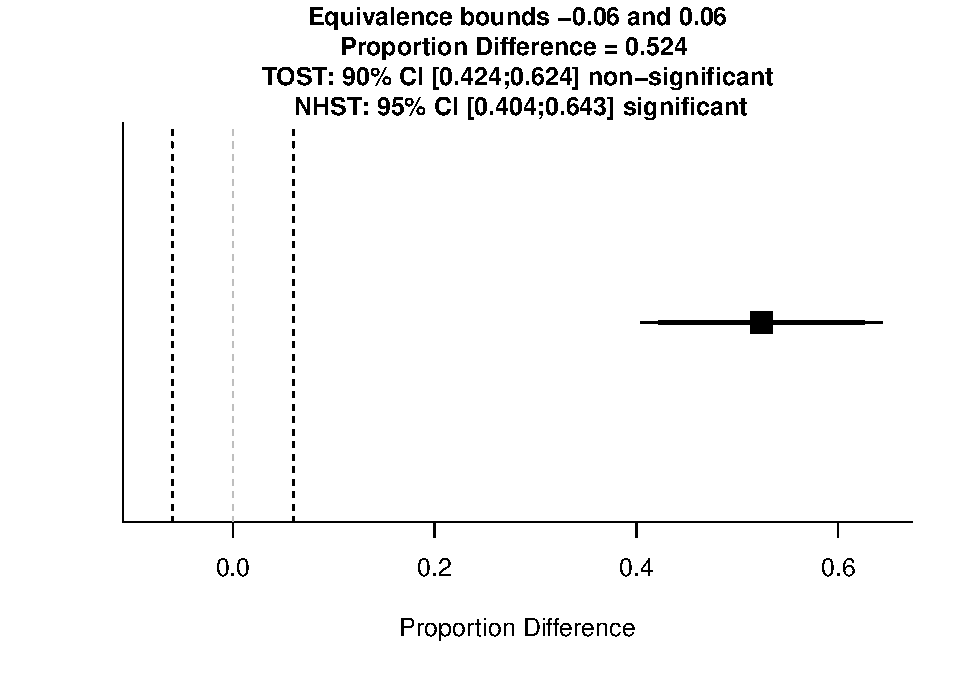
\includegraphics{manuscript_files/figure-latex/unnamed-chunk-3-1.pdf}
\caption{\label{fig:unnamed-chunk-3}Positive result rates for standard reports and Registered Reports. Error bars indicate 95\% confidence intervals around the observed positive result rate.}
\end{figure}

\hypertarget{exploratory-analyses}{%
\subsection{Exploratory Analyses}\label{exploratory-analyses}}

As expected, direct replications were much more common among RRs than SRs: 41 out of 71 RRs (\(57.75\%\)), but only 4 out of 152 SRs (\(2.63\%\)) were classified as direct replications of previously published work.
However, this difference cannot account for the stark overall difference between SRs and RRs described above:
Although replication RRs in our sample indeed had a lower positive result rate than original RRs (see Table 1), the difference between original SRs and original RRs -- \(45.95\%\) -- was still significantly different from 0 (\(\chi^2 = 46.28\), \(p < .001\)) and not statistically equivalent to a range between \(-6\%\) and \(6\%\) (\(z = 4.31\), \(p > .999\)), both at \(\alpha = 5\%\).

\begin{table}[tbp]
\begin{center}
\begin{threeparttable}
\caption{\label{tab:unnamed-chunk-5}Positive results in original studies vs replication studies}
\begin{tabular}{lrrrrrrrr}
\toprule
 & \multicolumn{4}{c}{original studies} & \multicolumn{4}{c}{replication studies} \\
\cmidrule(r){2-5} \cmidrule(r){6-9}
 & n & supported & \% & 95\% CI & n & supported & \% & 95\% CI\\
\midrule
SRs & 148 & 142 & 95.95 & 91.39; 98.50 & 4 & 4 & 100.00 & 39.76; 100.00\\
RRs & 30 & 15 & 50.00 & 31.30; 68.70 & 41 & 16 & 39.02 & 24.20; 55.50\\
\bottomrule
\addlinespace
\end{tabular}
\begin{tablenotes}[para]
\normalsize{\textit{Note.} SRs = standard reports, RRs = Registered Reports}
\end{tablenotes}
\end{threeparttable}
\end{center}
\end{table}

Since our SR sample represents a direct replication of Fanelli (2010) for the discipline Psychiatry \& Psychology, another interesting question to ask is how our results compare to Fanelli's.
The difference between the positive result rate for SRs in our sample (\(96.05\%\)) and Fanelli's (\(91.49\%\)) is \(4.56\%\). This difference is not significantly different from 0 in a two-sided proportions test (\(\chi^2 = 1.91\), \(p= .167\)) but also not statistically equivalent to a range between \(-6\%\) and \(6\%\) (\(z = -3.73\), \(p= .306\)), both at \(\alpha = 5\%\).
In other words, we can neither reject the hypothesis that the positive result rates of the two populations are the same, nor that there is a difference of at least \(\pm 6\%\) between them.
The data are inconclusive.

Finally, we analysed the language that was used to introduce or signal hypotheses in RRs.
Does Fanelli's search phrase \enquote{test\(^\ast\) the hypothes\(^\ast\)} capture hypothesis-testing RRs reasonably well?
The answer is a resounding \enquote{no}:
Searching the abstracts, titles, and keywords of the RR sample showed that only 2/71 RRs would have been detected with this search phrase.
Which analogous hypothesis-introduction phrases are used in RRs, and can they be summarised in a convenient way?
To get an overview, we stripped the hypothesis quotes of RRs from all content-specific information and extracted \enquote{minimal} phrases that most distinctively indicated that a hypothesis was being described.
For example, from the hypothesis quote \enquote{(f)or Study 1, we predicted that participants reading about academic (vs.~social) behaviors would show a better anagram performance} we extracted the hypothesis-introduction phrase \enquote{predicted that}.

For the majority of RRs (49), we identified one hypothesis-introduction phrase; the remaining ones used two (16 RRs), three (4 RRs), or four (1 RR) different phrases or had no identifiable hypothesis introduction (1 RR).
In this total set of 97 hypothesis introductions, we found 64 unique phrases, showing substantial linguistic variation (see Tables 2 and 3).
In order to condense the information further, we listed all unique word stems (e.g., the word stem \enquote{hypothes\(^\ast\)} captures the words \enquote{hypothesis}, \enquote{hypotheses}, \enquote{hypothesize}, \enquote{hypothesized}, and so on) and analysed their frequency among all hypothesis introductions.
Excluding words that are common but too unspecific by themselves, such as \enquote{that}, \enquote{to}, or \enquote{whether}, the five most frequent word stems were \enquote{hypothes\(^\ast\)} (34 occurrences), \enquote{replicat\(^\ast\)} (24), \enquote{test\(^\ast\)} (20), \enquote{examine\(^\ast\)} (8), and \enquote{predict\(^\ast\)} (8).
Clearly \enquote{test\(^\ast\)} and \enquote{hypothes\(^\ast\)} are quite popular, yet they co-occurred only 8 times and more than half of all hypothesis introductions (51/97) contained neither word. Interestingly, the frequency of these two words differed between original studies and direct replications: 30 out of 43 (\(69.77\%\)) hypothesis introductions found in original RRs contained either \enquote{test\(^\ast\)} or \enquote{hypothes\(^\ast\)} or both, while only 16 out of 54 (\(29.63\%\)) hypothesis introductions in direct replication RRs did.

We noticed that direct replication RRs generally tended to use different language to describe their hypothesis (or rather their goal). As the high frequency of the word stem \enquote{replicat\(^\ast\)} suggests, these studies were often not framed as new tests of a previously tested hypothesis, but as attempts to replicate a previously documented effect or to repeat a previously conducted experiment.
Tables 2 and 3 list all unique hypothesis introductions and their frequency for original RRs and direct replication RRs, respectively, grouped by the five most frequent word stems (\enquote{hypothes\(^\ast\)}, \enquote{replicat\(^\ast\)}, \enquote{test\(^\ast\)}, \enquote{examine\(^\ast\)}, \enquote{predict\(^\ast\)}).
Using five as a cutoff value is an arbitrary decision, but we believe that it strikes a reasonable balance between condensing the information and doing the variance of the data justice.

\begin{table}[tbp]
\begin{center}
\begin{threeparttable}
\caption{\label{tab:unnamed-chunk-9}Hypothesis introduction phrases in original Registered Reports (testing new hypotheses)}
\footnotesize{
\begin{tabular}{llrrr}
\toprule
 &  & \multicolumn{3}{c}{source} \\
\cmidrule(r){3-5}
core word(s) & introduction phrase & abstract & full text & total\\
\midrule
hypothes*, test* &  & 3 & 2 & 5\\
 & test of ... hypotheses & 0 & 1 & 1\\
 & test of ... hypothesis & 1 & 0 & 1\\
 & test the hypothesis that & 1 & 0 & 1\\
 & tested ... hypotheses & 0 & 1 & 1\\
 & tested the hypothesis that & 1 & 0 & 1\\ \midrule
hypothes* &  & 5 & 12 & 17\\
 & (Hypothesis 1) & 0 & 1 & 1\\
 & Hypothesis 1 (H1): & 0 & 2 & 2\\
 & Hypothesis 1: & 0 & 1 & 1\\
 & Hypothesis 1a (H1a): & 0 & 1 & 1\\
 & hypothesis was & 0 & 1 & 1\\
 & Hypothesis: & 0 & 1 & 1\\
 & hypothesize that & 0 & 3 & 3\\
 & hypothesized that & 4 & 2 & 6\\
 & registered ... hypotheses & 1 & 0 & 1\\ \midrule
test* &  & 5 & 2 & 7\\
 & test if & 0 & 1 & 1\\
 & test whether & 1 & 1 & 2\\
 & tested whether & 2 & 0 & 2\\
 & testing & 1 & 0 & 1\\
 & to ... test & 1 & 0 & 1\\ \midrule
test*, predict* & test ... prediction & 0 & 1 & 1\\ \midrule
predict* &  & 4 & 0 & 4\\
 & had ... predictions & 1 & 0 & 1\\
 & predicted that & 2 & 0 & 2\\
 & predicts that & 1 & 0 & 1\\ \midrule
examin* &  & 5 & 0 & 5\\
 & examine whether & 2 & 0 & 2\\
 & examined & 1 & 0 & 1\\
 & examined whether & 1 & 0 & 1\\
 & to examine & 1 & 0 & 1\\ \midrule
(other) &  & 0 & 5 & 5\\
 & (H1) & 0 & 1 & 1\\
 & expected that & 0 & 1 & 1\\
 & if ... then & 0 & 1 & 1\\
 & predication that & 0 & 1 & 1\\
 & we expect & 0 & 1 & 1\\
\bottomrule
\addlinespace
\end{tabular}
}
\begin{tablenotes}[para]
\normalsize{\textit{Note.} This table contains 44 hypothesis introduction phrases from 30 Registered Reports: 19 papers contributed one phrase each, 9 papers contributed two each, one contributed three, and one contributed four.}
\end{tablenotes}
\end{threeparttable}
\end{center}
\end{table}

\begin{table}[tbp]
\begin{center}
\begin{threeparttable}
\caption{\label{tab:unnamed-chunk-10}Hypothesis introduction phrases in replication Registered Reports (testing previously studied hypotheses)}
\footnotesize{
\begin{tabular}{llrrr}
\toprule
 &  & \multicolumn{3}{c}{source} \\
\cmidrule(r){3-5}
core word(s) & introduction phrase & abstract & full text & total\\
\midrule
hypothes*, test* &  & 2 & 1 & 3\\
 & test ... hypotheses & 0 & 1 & 1\\
 & test ... hypothesis & 1 & 0 & 1\\
 & tested ... hypotheses & 1 & 0 & 1\\ \midrule
hypothes*, predict* & hypotheses predicted & 1 & 0 & 1\\ \midrule
hypothes*, examin* & examined ... hypothesis & 1 & 0 & 1\\ \midrule
hypothes* &  & 2 & 5 & 7\\
 & according to ... hypothesis & 0 & 1 & 1\\
 & Hypotheses & 0 & 1 & 1\\
 & Hypothesis 1 (H1): & 0 & 1 & 1\\
 & hypothesize that & 0 & 1 & 1\\
 & hypothesized that & 2 & 1 & 3\\ \midrule
test* &  & 4 & 0 & 4\\
 & testing whether & 2 & 0 & 2\\
 & to ... test & 1 & 0 & 1\\
 & to test & 1 & 0 & 1\\ \midrule
replicat* &  & 20 & 3 & 23\\
 & aim ... to replicate & 0 & 1 & 1\\
 & aim at replicating & 1 & 0 & 1\\
 & aimed to replicate & 0 & 1 & 1\\
 & attempted to replicate & 1 & 0 & 1\\
 & attempts to replicate & 1 & 0 & 1\\
 & conducted ... replication & 3 & 0 & 3\\
 & conducted ... replications & 2 & 0 & 2\\
 & performed ... replication & 2 & 0 & 2\\
 & present ... replication & 1 & 0 & 1\\
 & present ... replications & 1 & 0 & 1\\
 & replicated ... experiment & 1 & 0 & 1\\
 & replicating & 0 & 1 & 1\\
 & report ... replication attempt & 1 & 0 & 1\\
 & report ... replications & 2 & 0 & 2\\
 & sought to replicate & 3 & 0 & 3\\
 & we replicated & 1 & 0 & 1\\ \midrule
replicat*, examin* & critically examine and replicate & 1 & 0 & 1\\ \midrule
predict* & predicted that & 2 & 0 & 2\\ \midrule
examin* & examine whether & 0 & 1 & 1\\ \midrule
(other) &  & 4 & 6 & 10\\
 & establish whether & 0 & 1 & 1\\
 & H1 & 0 & 2 & 2\\
 & investigate if & 1 & 0 & 1\\
 & sought to reproduce & 1 & 0 & 1\\
 & suggests that & 2 & 0 & 2\\
 & we ... conducted & 0 & 1 & 1\\
 & we assume & 0 & 1 & 1\\
 & we expect & 0 & 1 & 1\\
\bottomrule
\addlinespace
\end{tabular}
}
\begin{tablenotes}[para]
\normalsize{\textit{Note.} This table contains 53 hypothesis introduction phrases from 40 Registered Reports. One additional RR had no codeable hypothesis introduction. 30 papers contributed one phrase each, 7 papers contributed two each, and three contributed three each.}
\end{tablenotes}
\end{threeparttable}
\end{center}
\end{table}

\hypertarget{discussion}{%
\section{Discussion}\label{discussion}}

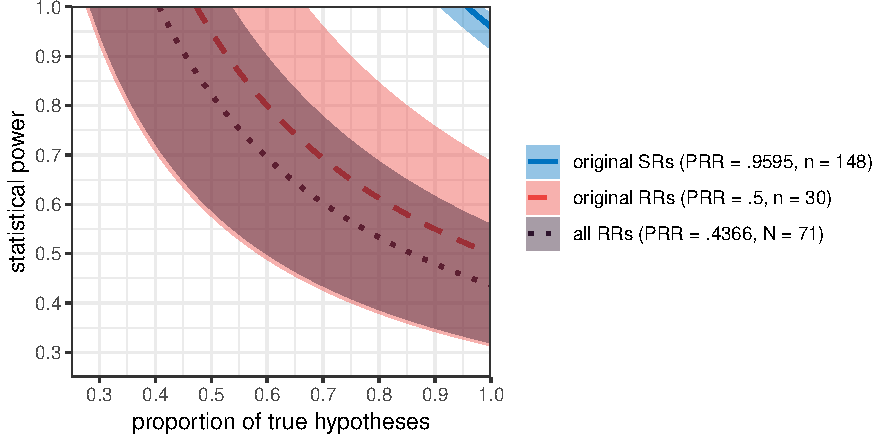
\includegraphics{manuscript_files/figure-latex/unnamed-chunk-11-1.pdf}

\hypertarget{references}{%
\section{References}\label{references}}

\setlength{\parindent}{-0.5in}
\setlength{\leftskip}{0.5in}

\hypertarget{refs}{}
\leavevmode\hypertarget{ref-Fanelli2010}{}%
Fanelli, D. (2010). "Positive" results increase down the hierarchy of the sciences. \emph{PLoS ONE}, \emph{5}(4), e10068. doi:\href{https://doi.org/10.1371/journal.pone.0010068}{10.1371/journal.pone.0010068}

\leavevmode\hypertarget{ref-Lakens2018a}{}%
Lakens, D., Scheel, A. M., \& Isager, P. M. (2018). Equivalence Testing for Psychological Research: A Tutorial. \emph{Advances in Methods and Practices in Psychological Science}, \emph{1}(2), 259--269. doi:\href{https://doi.org/10.1016/j.ympev.2015.01.015}{10.1016/j.ympev.2015.01.015}

\leavevmode\hypertarget{ref-Rohatgi2018}{}%
Rohatgi, A. (2018). \emph{WebPlotDigitizer - Web Based Plot Digitizer}. Austin, Texas, USA. Retrieved from \url{https://automeris.io/WebPlotDigitizer}

\leavevmode\hypertarget{ref-Fanelli2010}{}%
Fanelli, D. (2010). "Positive" results increase down the hierarchy of the sciences. \emph{PLoS ONE}, \emph{5}(4), e10068. doi:\href{https://doi.org/10.1371/journal.pone.0010068}{10.1371/journal.pone.0010068}

\leavevmode\hypertarget{ref-Lakens2018a}{}%
Lakens, D., Scheel, A. M., \& Isager, P. M. (2018). Equivalence Testing for Psychological Research: A Tutorial. \emph{Advances in Methods and Practices in Psychological Science}, \emph{1}(2), 259--269. doi:\href{https://doi.org/10.1016/j.ympev.2015.01.015}{10.1016/j.ympev.2015.01.015}

\leavevmode\hypertarget{ref-Rohatgi2018}{}%
Rohatgi, A. (2018). \emph{WebPlotDigitizer - Web Based Plot Digitizer}. Austin, Texas, USA. Retrieved from \url{https://automeris.io/WebPlotDigitizer}

\end{document}
